\chapter{Discussion}
Please tell more about conclusion and how to the next work of this study.

\section{Andi Muhammad Aslam/1164064}
\subsection{Teori}
\begin{enumerate}
\item Jelaskan kenapa file teks harus di lakukan tokenizer.
\subitem Tahap Tokenizing adalah tahap pemotongan string input berdasarkan tiap kata yang menyusunnya. Tokenisasi secara garis besar memecah sekumpulan karakter dalam suatu teks ke dalam satuan kata, bagaimana membedakan karakter-karakter tertentu yang dapat diperlakukan sebagai pemisah kata atau bukan. Sebagai contoh karakter whitespace, seperti enter, tabulasi, spasi dianggap sebagai pemisah kata. Namun untuk karakter petik tunggal (‘), titik (.), semikolon (;), titk dua (:) atau lainnya, dapat memiliki peran yang cukup banyak sebagai pemisah kata.
\begin{figure}[!htbp]
	\centerline{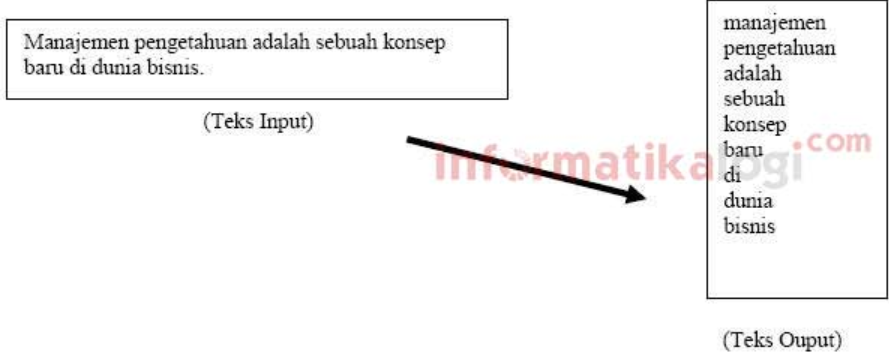
\includegraphics[width=1\textwidth]{figures/andi/7-1.PNG}}
	\caption{Tokenizer}
	\label{c7_1}
\end{figure}

\item Jelaskan apa itu Deep Learning.
\subitem Deep Learning adalah salah satu jenis algoritma jaringan saraf tiruan yang menggunakan metadata sebagai input dan mengolahnya menggunakan sejumlah lapisan tersembunyi (hidden layer) transformasi non linier dari data masukan untuk menghitung nilai output. Algortima pada Deep Learning memiliki fitur yang unik yaitu sebuah fitur yang mampu mengekstraksi secara otomatis.
\item Jelaskan apa itu Deep Neural dan bedanya dengan Deep Learning.
\begin{itemize}
\item Deep Neural Network atau DNN merupakan algoritma yang berbasis neural network yang digunakan untuk mengambil keputusan.
\item Yang membedakan Deep Learning dengan  Deep Neural Network (DNN) adalah DNN merupakan algoritma yang digunakan pada Deep Learning, sedangkan Deep Learning merupakan model yang menggunakan algoritma DNN.
\end{itemize}
\end{enumerate}